\documentclass[11pt]{article}

% Mathematical typesetting
\usepackage{amsmath}
\usepackage{amsthm}
\usepackage{amssymb}
\usepackage{gensymb}
\usepackage{bbm}

% Document formatting
\usepackage[utf8]{inputenc}
\usepackage{comment}
\usepackage{enumitem}
\usepackage{hyperref}
\usepackage{csquotes}
\usepackage{abstract}
\usepackage{array}
\usepackage{float}

\usepackage{pgfplots}
\usepgfplotslibrary{fillbetween}


%% Remove abstract text
\renewcommand{\abstractname}{\vspace{-\baselineskip}} 

\usepackage[]{geometry}
\geometry{margin=1in, headsep=0.25in}
\newlength{\tabcont}
\setlength{\parindent}{0.0in}
\setlength{\parskip}{0.05in}
\usepackage{framed}
\usepackage[most]{tcolorbox}
\usepackage{xcolor}

\newtheoremstyle{mystyle}{}{}{}{}{\bfseries}{:}{ }{\thmname{#1}\thmnumber{ #2}\thmnote{ (#3)}}
  
\theoremstyle{mystyle}
\newtheorem{thm}{Theorem}[section]
\newtheorem{lm}{Lemma}[section]
\newtheorem{defn}{Definition}[section]
\newtheorem{note}{Note}[section]

\newtheorem{protoexamp}{Example}[section]
\newenvironment{examp}
{\colorlet{shadecolor}{orange!15}\begin{shaded}\begin{protoexamp}}
{\end{protoexamp}\end{shaded}}

\newtheorem{protoexer}{Exercise}[section]
\newenvironment{exer}
{\colorlet{shadecolor}{blue!15}\begin{shaded}\begin{protoexer}}
{\end{protoexer}\end{shaded}}

\title{\textbf{Notes on Functional Analysis}}
\author{Henry Smith}
\date{\today}

\begin{document}

\maketitle
\begin{abstract}
    These notes are prepared from my reading of \textit{Introductory Functional Analysis with Applications} by Erwin Kreyszig. They are intended to serve as an aid for my understanding the book content. I do not guarantee their accuracy, and they do not reflect the accuracy of the book.
\end{abstract}

\newpage

\tableofcontents

\newpage

\section{Metric Spaces}

\subsection{Metric Spaces: Definition and Examples}

\begin{defn}[Metric Space]\label{metric}
A \textbf{metric space} is a pair $(X, d)$, where $X$ is a set and $d: X \times X \rightarrow \mathbb{R}_+$ is a \textbf{metric} on $X$. The metric $d$ must satisfy the following for all $x, y, z \in X$:
\begin{enumerate}
    \item $d(x, y) = 0 \iff x = y$
    \item $d(x, y) = d(y, x)$  \quad (symmetry)
    \item $d(x, z) \leq d(x, y) + d(y, z)$ \quad (triangle inequality)
\end{enumerate}
\end{defn}

A metric can be thought of as a measure of distance between any two elements $x, y \in X$. To illustrate this point, we provide some examples of metric spaces:

\begin{examp}[The real line $\mathbb{R}$] Let $X = \mathbb{R}$ and $d(x, y) := |x - y|$. Then $(X, d)$ is a metric space. This is our most classical notion of distance.
\end{examp}

\begin{examp}[The complex plane $\mathbb{C}$] Similarly, we let $X= \mathbb{C}$ and $d(x, y) := |x - y|$ for $x, y \in \mathbb{C}$. Recall that for $x = a + bi$, the modulus of $x$ is defined $|x| = \sqrt{a^2 + b^2}$. Then $(X, d)$ is a metric space.

\end{examp}

\begin{examp}[The Euclidean space $\mathbb{R}^n$, unitary space $\mathbb{C}^n$] For $X = \mathbb{R}^n$, we define $d(x, y) := \sqrt{(\xi_1 - \eta_1)^2 + \ldots + (\xi_n - \eta_n)^2 }$, where $x = (\xi_1, \ldots, \xi_n), y = (\eta_1, \ldots, \eta_n) \in \mathbb{R}^n$. $(X, d)$ defines the Euclidean metric space.\newline
Similarly, let $X = \mathbb{C}^n$ and define $d(x, y) := \sqrt{|\xi_1 - \eta_1|^2 + \ldots + |\xi_n - \eta_n|^2}$ for $x, y \in \mathbb{C}^n$. $(X, d)$ defines the unitary metric space.
\end{examp}

These are perhaps the most benign metric spaces that we can conjure from memory. Before presenting more exotic examples of metric spaces, we first discuss a few additional results:

\begin{lm}[Generalized Triangle Inequality]
Let $(X, d)$ be a metric space with $x_1, \ldots, x_n \in X$. Then it holds that
\begin{align*}
    d(x_1, x_n) \leq d(x_1, x_2) + \ldots + d(x_{n-1}, x_n).
\end{align*}
\end{lm}
This follows from an elementary induction argument.

\begin{defn}[Subspace]
Let $(X, d)$ be a metric space and $Y \subset X$ a subset of $X$. Then we can define a metric $\tilde{d}$ on $Y$ according to $\tilde{d} = d|_{Y \times Y}$. This is called the metric induced on $Y$ by $d$.
\end{defn}

The following are important examples of metric spaces that will be relevant throughout the remainder of our studies:
\begin{examp}[The sequence space $\ell^p$]\label{ellp}
For fixed $p \geq 1$, we define the space $\ell^p$ to consist of those complex sequences $x = (\xi_n)_{n=1}^{\infty} \subset \mathbb{C}$ such that
\begin{align*}
    \sum_{n=1}^{\infty}|\xi_n|^p < \infty.
\end{align*}
The metric defined on $\ell^p$ is 
\begin{align*}
    d(x, y) = \left( \sum_{n=1}^{\infty} |\xi_n - \eta_n|^p \right)^{1/p}, \qquad x = (\xi_n), \  y = (\eta_n) \in \ell^p.
\end{align*}
One can verify that indeed $d(x, y) < \infty$ using the \textit{Minkowski inequality}:
\begin{align*}
    \left( \sum_{n=1}^{\infty} | \xi_n + \eta_n|^p  \right)^{1/p} \leq \left( \sum_{n=1}^{\infty} | \xi_n|^p  \right)^{1/p} + \left( \sum_{n=1}^{\infty} |\eta_n|^p  \right)^{1/p}.
\end{align*}
Then $(\ell^p, d)$ defines a metric space. In the special case of $p = 2$, this is a \textbf{Hilbert space} (see Section \ref{}).
\end{examp}

\begin{examp}[The sequence space $\ell^{\infty}$]
Similar to the space considered in Example \ref{ellp}, we let $\ell^{\infty}$ be the set of all bounded sequences in $\mathbb{C}$. That is,
\begin{align*}
    \ell^{\infty} = \{ x = (\xi_n) \subset \mathbb{C} \ | \  | \xi_n | \ \leq c_x \ \text{for some $c_x \in \mathbb{R}_+$} \}.
\end{align*}
The metric we define on $\ell^{\infty}$ is $d(x, y) = \sup_{n \in \mathbb{N}} |\xi_n - \eta_n |$. $(\ell^{\infty}, d)$ defines a metric space.
\end{examp}

\begin{examp}[The function space $C{[a,b]}$]\label{contfun}
Let $X$ be the set of all real-valued continuous functions defined on the interval $[a, b]$. Then for each $x(t), y(t) \in X$, we define the metric $d(x, y) := \max_{t \in [a, b]} | x(t) - y(t) |$.\newline 
One should notice that we use \enquote{max} rather than \enquote{sup} in our definition of the metric $d$. This is because $f(t) = |x(t) - y(t)|$ is continuous on the closed interval $[a, b]$ and thus attains its maximum on this interval (the Weierstrass Extreme Value Theorem).\newline
This defines the metric space $C[a, b]$.
\end{examp}

\begin{examp}[The discrete metric space]\label{discretemetric}
For any set $X$, define the metric $d$ such that
\begin{align*}
    d(x, y) = 
    \begin{cases}
    1 & \text{if $x=y$} \\
    0 & \text{otherwise}
    \end{cases}.
\end{align*}
Then $(X, d)$ is called the \textbf{discrete metric space}.
\end{examp}

\begin{exer}
If $A$ is the subspace of $\ell^{\infty}$ consisting of all zeros and ones, what is the induced metric on $X$?\newline
The induced metric $\tilde{d}$ on $A$ is the discrete metric (see Example \ref{discretemetric}).
\begin{proof}
Let $x = (\xi_n), y = (\eta_n) \in A$. Then if $x \neq y$, it must be the case that $|\xi_j - \eta_j| = 1$ for some $j \in \mathbb{N}$. By the definition of $(\ell^{\infty}, d)$, this implies $\tilde{d}(x, y) = 1$. Also, by the properties of a metric space, we know $\tilde{d}(x, x) = 0$. We deduce that $\tilde{d}$ is the discrete metric.
\end{proof}
\end{exer}

\begin{exer}
Show that a metric on the space $X$ from Example \ref{contfun} is 
\begin{align*}
    \tilde{d}(x, y) = \int_a^b |x(t) - y(t)| dt.
\end{align*}

\begin{proof}
First, notice that since $x, y \in X$, then $|x - y| \in X$. That is, $|x(t) - y(t)|$ is continuous over $[a, b]$, and is thus Riemann integrable. This means that $\tilde{d}$ is well-defined. Similarly, we have
\begin{enumerate}
    \item $|x(t) - y(t)| \geq 0, \ t \in [a, b] \implies \tilde{d}(x, y) = \int_a^b |x(t) - y(t)| dt \geq 0$
    \item $|x(t) - y(t)| \leq c, \ \forall t \in [a, b]$ for some $c \in \mathbb{R}_+$ $\implies \tilde{d}(x, y) \leq c \cdot (b -a) \in \mathbb{R}_+$
\end{enumerate}
Therefore, it is indeed the case that $\tilde{d}: X \times X \rightarrow \mathbb{R}_+$.\newline
To verify axiom (1), we clearly see that $x = y$ implies $\tilde{d}(x, y) = 0$. For the opposite implication, suppose $x(t_0) \neq y(t_0)$ for some $t_0 \in [a, b]$. Without loss of generality, suppose $t_0 \notin \{a, b\}$. Then by the continuity of $x$ and $y$, this implies that $|x(t) - y(t)| > 0$ for all $t \in [t_0 - \varepsilon, t_0 + \varepsilon] \subseteq [a, b]$, where $\varepsilon > 0$ is chosen to be sufficiently small. Accordingly, we have
\begin{align*}
    &\tilde{d}(x, y) = \underbrace{\int_a^{t_0 - \varepsilon} |x(t) - y(t)| dt}_{\geq 0} + \underbrace{\int_{t_0 - \varepsilon}^{t_0 + \varepsilon} |x(t) - y(t)| dt}_{> 0} + \underbrace{\int_{t_0 - \varepsilon}^{b} |x(t) - y(t)| dt}_{\geq 0}\\
    \implies&\tilde{d}(x, y) > 0.
\end{align*}
Symmetry (2) of the metric $\tilde{d}$ follows from the properties of the absolute value.\newline
Finally, to prove the triangle inequality (3), we have that for $x, y, z$ continuous functions on $[a, b]$
\begin{align*}
    \tilde{d}(x, z) &= \int_a^b | x(t) - z(t) | dt \leq \int_a^b \bigg( | x(t) - y(t) | +  | y(t) - z(t) |\bigg) dt\\
    &= \int_a^b | x(t) - y(t) | dt + \int_a^b | y(t) - z(t) | dt\\
    &= \tilde{d}(x, y) + \tilde{d}(y, z).
\end{align*}
\end{proof}
\end{exer}

\begin{exer}
Show that nonnegativity of a metric follows from axioms (1) - (3).

\begin{proof}
Let $(X, d)$ be a metric space and $x, y \in X$ arbitrary points. Then by (3) we have
\begin{align*}
    d(x, x) \leq d(x, y) + d(y, x).
\end{align*}
Property (1) implies
\begin{align*}
    0 \leq d(x, y) + d(y, x).
\end{align*}
And property (2) implies
\begin{align*}
    0 \leq 2d(x, y) \iff 0 \leq d(x, y).
\end{align*}
\end{proof}
\end{exer}

\begin{exer}

Define $s$ to be the space of all (bounded or unbounded) sequences of complex numbers and the metric $d$ defined by
\begin{align*}
    d(x, y) = \sum_{n=1}^{\infty} \frac{1}{2^n} \frac{|\xi_n - \eta_n|}{1 + |\xi_n - \eta_n|}, \qquad x = (\xi_n), \ y= (\eta_n) \in s.
\end{align*}
Show that we can obtain another metric by replacing $(1/2^n)$ with $(\mu_n), \ \mu_n > 0$ such that $\sum \mu_n$ converges.
\begin{proof}
First, we point out that $\mu_n \cdot \frac{|\xi_n - \eta_n|}{1 + |\xi_n - \eta_n|} \geq 0$ for each $n \in \mathbb{N}$, and so $\tilde{d}(x, y) = \sum_{n=1}^{\infty} \mu_n \cdot \frac{|\xi_n - \eta_n|}{1 + |\xi_n - \eta_n|} \geq 0$. Also we notice that $\mu_n \cdot \underbrace{\frac{|\xi_n - \eta_n|}{1 + |\xi_n - \eta_n|}}_{ < 1} < \mu_n$ for each $n \in \mathbb{N}$, and so $\tilde{d}(x, y) = \sum_{n=1}^{\infty} \mu_n \cdot \frac{|\xi_n - \eta_n|}{1 + |\xi_n - \eta_n|} < \sum_{n=1}^{\infty} \mu_n < \infty$.\newline
Now, for (1) we have 
\begin{align*}
    &\tilde{d}(x, y) = 0 \iff \sum_{n=1}^{\infty} \underbrace{\mu_n \cdot \frac{|\xi_n - \eta_n|}{1 + |\xi_n - \eta_n|}}_{\geq 0} = 0 \iff \mu_n \cdot \frac{|\xi_n - \eta_n|}{1 + |\xi_n - \eta_n|} = 0, \ n \in \mathbb{N}\\
    \iff&  \frac{|\xi_n - \eta_n|}{1 + |\xi_n - \eta_n|} = 0, \ n \in \mathbb{N} \iff x = y.
\end{align*}
(2) follows simply from the properties of the modulus function.\newline
Finally, for the triangle inequality (3), we let $z = (\gamma_n) \in s$ and use the result from pp. 10 - 11:
\begin{align*}
    &\frac{|\xi_n - \gamma_n|}{1 + |\xi_n - \gamma_n|} \leq \frac{|\xi_n - \eta_n|}{1 + |\xi_n - \eta_n|} + \frac{|\eta_n - \gamma_n|}{1 + |\eta_n - \gamma_n|}, \quad n \in \mathbb{N}\\
    \iff&\mu_n \cdot \frac{|\xi_n - \gamma_n|}{1 + |\xi_n - \gamma_n|} \leq \mu_n \cdot \frac{|\xi_n - \eta_n|}{1 + |\xi_n - \eta_n|} + \mu_n \cdot \frac{|\eta_n - \gamma_n|}{1 + |\eta_n - \gamma_n|}, \quad n \in \mathbb{N}\\
    \implies& \sum_{n=1}^{\infty} \mu_n \cdot \frac{|\xi_n - \gamma_n|}{1 + |\xi_n - \gamma_n|} \leq \sum_{n=1}^{\infty} \mu_n \cdot \frac{|\xi_n - \eta_n|}{1 + |\xi_n - \eta_n|} + \sum_{n=1}^{\infty} \mu_n \cdot \frac{|\eta_n - \gamma_n|}{1 + |\eta_n - \gamma_n|}\\
    \iff& \tilde{d}(x, z) \leq \tilde{d}(x, y) + \tilde{d}(y, z).
\end{align*}
We deduce $(s, \tilde{d})$ is a metric space.
\end{proof}
\end{exer}

\begin{exer}
The \textbf{diameter} $\delta(A)$ of a nonempty set $A$ in a metric space $(X, d)$ is defined to be 
\begin{align*}
    \delta(A) = \sup_{x, y\in A} d(x, y).
\end{align*}
$A$ is said to be \textbf{bounded} if $\delta(A) < \infty$. Prove each of the following:
\begin{enumerate}
    \item $A \subset B$ implies $\delta(A) \leq \delta(B)$.
    \item $\delta(A) = 0 \iff$ $A$ consists of a single point.
\end{enumerate}

\begin{proof}
(1) This follows from the properties of the the supremum. Namely, 
\begin{align*}
    &C_1=\{d(x, y) \ | \ x, y \in A \} \subset C_2=\{d(x, y) \ | \ x, y \in B \}\\
    \implies& \sup C_1 \leq \sup C_2\\
    \iff& \delta(A) \leq \delta(B).
\end{align*}
(2) 
\begin{align*}
    &\delta(A) = 0 \iff \sup_{x, y\in A} d(x, y) = 0 \iff d(x, y) = 0, \ \forall x, y \in A\\
    &\iff\text{A consists of a single point}
\end{align*}
\end{proof}
\end{exer}

\begin{exer}
The \textbf{distance} $D(A, B)$ between two nonempty subsets $A$ and $B$ of a metric space $(X, d)$ is defined to be 
\begin{align*}
   D(A, B) = \inf_{\substack{a \in A\\b \in B}} d(a, b). 
\end{align*}
Show each of the following:
\begin{enumerate}
    \item $D$ does \textit{not} define a metric on the power set of $X$.
    \item If $A \cap B \neq \varnothing$, then $D(A, B) = 0$. What about the converse?
\end{enumerate}

\begin{proof}
(1) Let $P, Q \in 2^X$ such that $P \neq Q$ and $P \cap Q \neq 
\varnothing$. Notice that $d$ is a metric, and so $d(p, q) \geq 0, \ \forall p \in P, \ \forall q \in Q$. This implies $D(P, Q) \geq 0$. Moreover, $P \cap Q \neq \varnothing$ implies $D(P, Q) \leq 0$. Altogether, we have shown $D(P, Q) = 0$ but $P \neq Q$. Therefore, we conclude $D$ does not define a metric.\newline
(2) Since $A \cap B \neq \varnothing$, then $0 \in \{ d(a, b) \ | \ a \in A, \ b \in B\}$. This tells us that $D(A, B) \geq 0$. And by our argument from (1), $d(a, b) \geq 0, \ \forall a \in A, \ \forall b \in B$, which implies $D(A, B) = \inf_{\substack{a \in A\\b \in B}} d(a, b) \geq 0$. We conclude $D(A, B) = 0$.\newline
The converse is not true. Consider the Euclidean metric space $(\mathbb{R}^2, d)$. Let $A = \{(x, 0) \ | \ x > 0 \}$ be the positive $x$-axis and $B = \{(x, y) \ | \ x >0, \ y \geq x^{-1} \}$ the region bounded by the curve $y = x^{-1}$. Since $x^{-1} > 0$ for every $x > 0$, then $A \cap B = \varnothing$. Consider the sequence $(a_n) \subset A$ defined $a_n = (n, 0)$ as well as the sequence $(b_n) \subset B$ defined $b_n = (n, n^{-1})$. Then $d(a_n, b_n) = n^{-1}$ for all $n \in \mathbb{N}$, which proves that $D(A, B) = \inf_{\substack{a \in A\\b \in B}} d(a, b) \leq 0$. By nonnegativity of the metric $d$, we conclude $D(A, B) = 0$ but $A \cap B = \varnothing$.
\end{proof}

% Add plot
\begin{center}
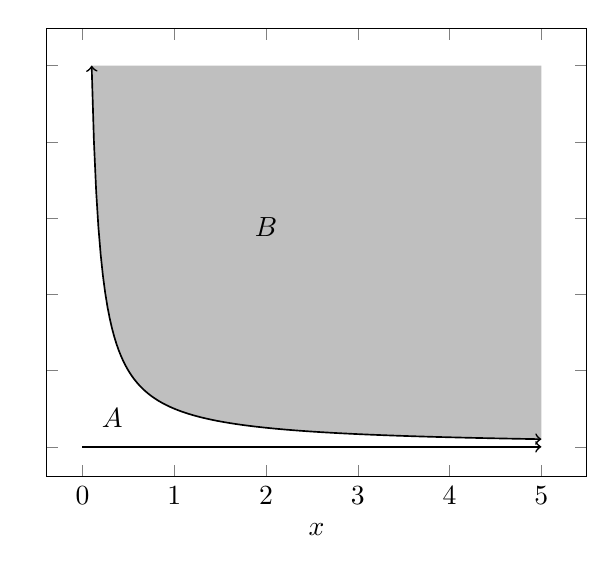
\begin{tikzpicture}
\begin{axis}[samples=200, xlabel={$x$}, yticklabels={}]
\addplot[<->, semithick][name path=f, domain=.1:5] {1/x};
\node[label={$B$}] at (axis cs:2,5) {};
\path[name path=axis] (axis cs:0.1,10) -- (axis cs:5,10);
\addplot[gray!50] fill between[of=f and axis];
\node[circle, label={45:$A$}] at (axis cs:0,0) {};
\draw[->, semithick] (axis cs:0,0) -- (axis cs:5,0);
\end{axis}
\end{tikzpicture}
\end{center}
\end{exer}

\newpage
\begin{exer}
The \textbf{distance} $D(x, B)$ from a point $x$ to a nonempty subset $B$ of a metric space $(X, d)$ is defined to be
\begin{align*}
    D(x, B) = \inf_{b \in B} d(x, b).
\end{align*}
Show that for any $x, y \in X$,
\begin{align*}
    |D(x, B) - D(y, B)| \leq d(x, y).
\end{align*}
\begin{proof}
For each element $b \in B$, it holds that $d(x,b) \leq d(x, y) + d(y, b)$ by the triangle inequality. Consequently, we get the inequality 
\begin{align*}
    \inf_{b \in B} d(x, b) \leq d(x, y) + \inf_{b \in B} d(y, b) \iff D(x, B) - D(y, B) \leq d(x, y).
\end{align*}
By starting with $d(y, b) \leq d(y, x) + d(x, b)$, we similarly have $D(y, b) - D(x, b) \leq d(x, y)$. And so we conclude $|D(x, B) - D(y, B)| \leq d(x, y)$, as desired.
\end{proof}
\end{exer}

\subsection{Set Theory, Continuity, and Separability}


\end{document}